\chapter{Análisis general del proyecto}
	Para el desarrollo del sistema en su totalidad, se realizó el siguiente análisis general que define en su totalidad al proyecto.

	\section{Características}
		Para que el sistema se considere que ha cumplido con los objetivos planteados debe contar con las siguientes características dentro de su funcionalidad.
		\begin{itemize}			
			\item El sistema permitirá la búsqueda de platillos.
			\item El sistema permitirá obtener recomendaciones de acuerdo a las características de un platillo.
			\item El sistema obtendrá información de la interacción del usuario a través de evaluaciones explícitas, y conteo de clics implícitos hacia los platillos para obtener recomendaciones personalizadas para dicho usuario.
			\item El sistema permitirá el registro de usuarios finales.
			\item El sistema generará recomendaciones de platillos de acuerdo a la información proporcionada de los usuarios registrados, con base en sus evaluaciones y características.
			\item El sistema permitirá al usuario agregar nuevos platillos que haya consumido en cierto restaurante.
			\item El sistema permitirá al usuario administrar los platillos que agregó. 
		\end{itemize}

	\section{Restricciones}
		Debido a diferentes aspectos, el sistema contará con las siguientes restricciones.
		\begin{itemize}
			\item El sistema se verá limitado a las tecnologías empleadas para su desarrollo.
			\item El sistema puede verse limitado debido a la dependencia de fuentes de información externas.
			\item El sistema puede verse limitado en desempeño y precisión debido a la cantidad de información almacenada y a la complejidad del problema a resolver.
		\end{itemize} 

	\section{Estudio de factibilidad}
Después de definir la problemática presente y presentar la propuesta de solución, es  pertinente realizar un estudio de factibilidad para determinar la infraestructura tecnológica y la capacidad técnica que implica la implementación de la API en cuestión. Este análisis permite determinar las posibilidades de diseñar a API propuesta y su puesta en marcha. 
\\\\
A continuación se describen los aspectos que se toman en cuenta para este análisis.
\subsection{Factibilidad técnica }
Consiste en realizar una evaluación de la tecnología existente; este estudio está destinado a recolectar información sobre los componentes tecnológicos que posee este equipo de desarrollo y la posibilidad de utilizarlos en el desarrollo e implementación de este trabajo y de ser necesario, los requerimientos tecnológicos que deben ser adquiridos su desarrollo e implementación. 
\\\\
Hardware 
\\\\
Para el desarrollo de la API se cuentan con 3 computadoras personales, las cuales cuentan 
con las siguientes características:
\begin{itemize}
 \item MacBook Pro 13: 4 GB DDR3 RAM, Procesador Intel i5 a 2.5 GHz. S.O
 \item HP  8 GB DDR3 RAM, Procesador A10 2.1 GHz. S.O. Ubuntu 14.04.
 \item Acer 8 GB DDR3 RAM Procesador AMD A6 
\end{itemize}


Los módulos desarrollados para la primera parte del Trabajo Terminal serán expuestos de 
manera local, accediendo a ellos a través de una red local. Para la segunda entrega del 
Trabajo Terminal se tiene planeado exponerlos en un servidor, para lo cual se contará un 
servicio de hosting. No se incluirá en este documento la opción elegida para el hosting ni el 
costo del mismo, ya que no se sabe con exactitud cual se elegirá, a pesar de que se han 
tomado en cuenta varios, no se ha llegado a una decisió.
\newpage
Software  
\begin{itemize}
\item Java
\item Neo4j
\item Hibernate
\item JavaScript
\item HTML
\item Boostrap
\item Spring
\item Maven
\end{itemize}
Estas tecnologías son necesarias para el desarrollo de esta API. Cada una cumple con un  objetivo específico para las cuales fueron utilizadas, pero no son indispensables. No son indispensables, ya que se encuentran muchos otros lenguajes y frameworks con los cuales se pueden reemplazar estas tecnologías. 
\\\\
Costos 
\\\\
Los costos que generará el desarrollo de este framework se calcularon de la siguiente manera: 
\begin{itemize}
\item El manejo roles se repartió en el equipo, es decir, todos tuvieron que analizar, 
diseñar y desarrollar.  
\item Nos basamos en un sueldo promedio al cual aspiran estudiantes de la carrera de 
Ing. en Sistemas Computacionales, que es de \$ 80
\end{itemize}
Después de aclarar lo siguiente, los costos operacionales (mano de obra) se calcularon así:
\begin{itemize}
\item 3 personas que desarrollan diferentes actividades 
\item Cada uno gana \$80 la hora desarrollando la API 
\item Se toma en cuenta que se  trabajan los 7 días de la semana 4 horas cada uno de ellos, así: 
\end{itemize}
(\$80) * (4 hrs) * (250 dias) = \$80,000 
 
El precio estimado de este sistema es de \$80000 mx solamente tomando en cuenta la manos de obra, sin contemplar nuevos equipos, reuniones, transportes, comida y horas extras. 
\newpage
	\section{Metodología}
	\subsection{Descripción}
	  Para ese proyecto se plantea usar una metodología de prototipado evolutivo, que se caracteriza por que en su modelo de trabajo un prototipo es construido, probado y finalmente reconstruido las veces que sea necesario hasta que un prototipo aceptable es finalmente alcanzado del cual el sistema completo o producto puede ser totalmente desarrollado.

	  Este modelo funciona bien en escenarios donde no se conocen por completo los requerimientos. Así los prototipos, modelos de software con una funcionalidad limitada, permiten al usuario evaluar los propósitos del desarrollador y probarlos antes de su implementación. También ayuda a entender los requerimientos específicos del usuario y que no pudieron haber sido considerados por el desarrollador durante el diseño del sistema.

	\subsection{Prototipos esperados}
	  De acuerdo al modelo de desarrollo elegido, se han establecido los siguientes prototipos y sus alcances que se pueden observar en el cuadro~\ref{table:prototipos}

	  \begin{table}[h]
	  \begin{center}
	  \begin{tabular}{ | c | c | }
	    \toprule
	    	\textbf{Versión} & \textbf{Alcance} \\
	    \midrule
	    	Prototipo 1 & Obtener y abstraer los datos a utilizar\\
	    \midrule
	    	Prototipo 2 & Visualizar los datos en recomendaciones por contenido\\
	    \midrule
	    	Prototipo 3 & Obtener recomendaciones para diversos fines (sistemas híbridos) \\
	    \midrule
	    	Prototipo 4 & Desarrollar un sistema híbrido de recomendación para platillos y restaurantes. \\
	    \bottomrule
		\end{tabular}
	  \caption{Cuadro de prototipos esperados}
  	  \label{table:prototipos}
  	\end{center}
	\end{table}


	\section {Descripción y módulos del sistema}
% \section{¿Para qué sirve el sistema?}

  \subsection{Arquitectura general}
    \paragraph{Para desarrollar un sistema de recomendacion se han planteado los siguientes módulos funcionales de la API, el cual será utilizado por el desarrollador final para que, en conjunto con su aplicación final realice la integración de las funciones disponibles en el API junto al sistema de recomendación final. Esto se puede denotar en el siguiente diagrama.}

\newpage
    \begin{landscape}
      \begin{figure}[h!]
      \centering
      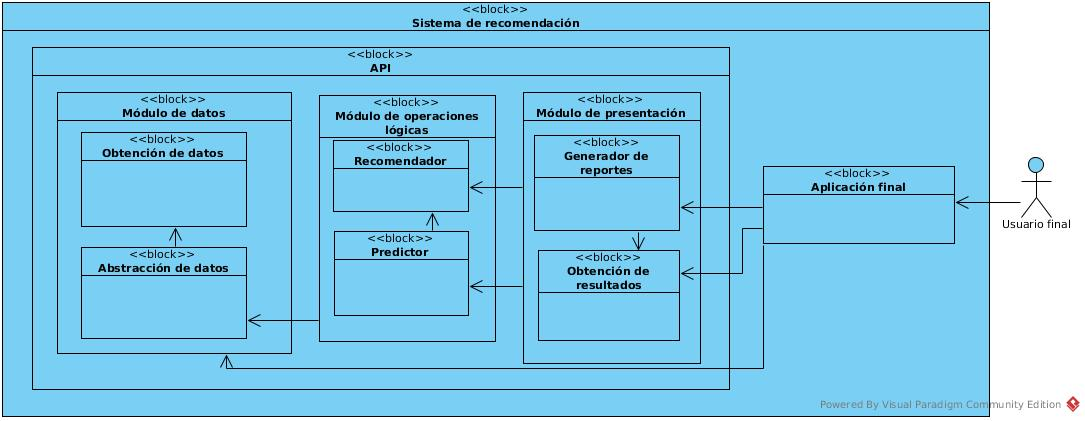
\includegraphics[width=22.5cm,height=12cm]{./images/architecture_diagram.jpg}
      \caption{Diagrama general del sistema}
    \end{figure}
    \end{landscape}
  \newpage

\paragraph{Cómo se apreciar en el diagrama, el sistema se encuentra dividido en tres módulos básicos además de la aplicación final que hace uso de los módulos de la API.}
    \begin{itemize}
    \item Módulo de datos
    \item Módulo de operaciones lógicas
    \item Módulo de presentación
    \item Caso de estudio ó aplicación final
  \end{itemize}

\subsection{Módulos de la API}
  \subsubsection{Módulo de abstracción de datos}
    \paragraph{Este módulo es el encargado de la obtención de datos para su adecuada manipulación dentro de los objetivos del sistema, es decir, permitirá el manejo de los datos estandarizandolos a un modelo de datos base que permitirá tener la funcionalidad del sistema de recomendación de manera adecuada. }
    \paragraph{Se presenta como un módulo conformado por diferentes interfaces de conexión para fuentes de datos, como pueden ser ficheros de texto o la conexión a un gestor de base de datos. Tiene una interacción directa con el módulo de operaciones lógicas dentro del sistema.}

  \subsubsection{Módulo de operaciones lógicas}
    \paragraph{El módulo de operaciones lógicas permitirá, haciendo uso de la información almacenada, obtener recomendaciones y predicciones de los diferentes artículos deacuerdo a diferentes clasificaciones con base en los principales tipos de recomendacion existentes: basados en contenido y colaborativos. Cabe destacar, la constante operación de este módulo para el aprendizaje y mejora constante de las recomendaciones.}

  \subsubsection{Módulo de presentación}
    \paragraph{Haciendo uso del módulo de operaciones lógicas, este módulo pretende brindar la funcionalidad de mostrar en forma de reportes tabulares, los resultados obtenidos de la recomendación al ser integrado en la aplicación final.}

\subsection{Aplicación final}
  \subsubsection{Definición}
    \paragraph{En este caso, la aplicación final hará uso de las funciones proporcionadas por los distintos módulos que conforman la API para obtener recomendaciones de los datos que pertenezcan a su caso de estudio. Interactúa directamente con el módulo de abstraccion de datos y con el módulo de presentación para hacer uso de la funcionalidad permitida por el API. En este caso, la aplicación final se verá reflejada en un sistema web que permita denotar la funcionalidad de la API para un conjunto de datos de platillos y restaurantes.}
	\section{Análisis y gestión de riesgos}
  \subsection{Definición y clasificación}
    El riesgo siempre implica una incertidumbre y una pérdida potencial, al identificar estos riesgos podemos determinar su naturaleza en tres tipos diferentes para este proyecto:
    \begin{itemize}
      \item Riesgos del proyecto
      \item Riesgos técnicos
      \item Riesgos de negocio
    \end{itemize}
    Así mismo, es necesario clasificar los riesgos existentes de acuerdo  a la probabilidad de que éstos ocurran. Para lo cual se utilizará los siguientes valores por convención.
    \begin{itemize}
      \item Muy bajo ( < 10\% )
      \item Bajo ( 10 - 25\% )
      \item Moderado (25 - 50\% )
      \item Alto (50 - 75\% )
      \item Muy Alto ( > 75\% )
    \end{itemize}
    Así mismo, todos los riegos depen categorizarse deacuero al impacto que pueden causar en el sistema en las siguientes categorías: Insignificante, Tolerable, Serio, Catastrófico; los planes de contingencia suelen ser desarrollados para aquellos riegos con probabilidad de moderada a muy alta y con un impacto serio o castastrófico.
    A continuación se plantean los riesgos identificados para el sistema general a lo largo del desarrollo del mismo y sus respectivos planes de acción.
    \newpage
    \begin{table}[b!]
    \centering
      \begin{tabular}{|p{3cm}|lllll}
        \hline
        \multicolumn{5}{|c|}{{\bf Tabla de Riesgos}} \\ 
        \hline
          \multicolumn{1}{|p{3cm}|}{{\bf Descripcion}} & 
          \multicolumn{1}{p{2cm}|}{{\bf Tipo de Riesgo}} & 
          \multicolumn{1}{p{2cm}|}{{\bf Valoración}} & 
          \multicolumn{1}{p{2cm}|}{{\bf Porcentaje}} & 
          \multicolumn{1}{p{5cm}|}{{\bf Plan de acción}} \\ 
        \hline
          \multicolumn{1}{|p{3cm}|}{Falta de presupuesto} & 
          \multicolumn{1}{p{2cm}|}{Proyecto} & 
          \multicolumn{1}{p{2cm}|}{Serio} & 
          \multicolumn{1}{p{2cm}|}{25\%} & 
          \multicolumn{1}{p{5cm}|}{Buscar un proceso de incubación en empresas como Apache, Eclipse y migrar la plataforma a servicios de hosting gratuitos como Heroku u Openshift.} \\ 
        \hline
          \multicolumn{1}{|p{3cm}|}{Falta por razones personales de miembros del equipo} & 
          \multicolumn{1}{p{2cm}|}{Proyecto} &
          \multicolumn{1}{p{2cm}|}{Serio} & 
          \multicolumn{1}{p{2cm}|}{25\%} & 
          \multicolumn{1}{p{5cm}|}{Rediseñar y adaptar las tareas con nuevos integrantes y habilitar forma de trabajo remota considerando fines de semana.} \\ 
        \hline
          \multicolumn{1}{|p{3cm}|}{Necesidad de escalabilidad de la plataforma} & 
          \multicolumn{1}{p{2cm}|}{Técnico} & 
          \multicolumn{1}{p{2cm}|}{Serio} & 
          \multicolumn{1}{p{2cm}|}{10\%} & 
          \multicolumn{1}{p{5cm}|}{Definir el tipo de escalabilidad a usar dependiendo los recursos monetarios existentes.} \\ 
        \hline
          %\multicolumn{1}{|p{3cm}|}{Ataques de Denegación de Servicios (DoS)} & 
          %\multicolumn{1}{p{2cm}|}{Técnico} & 
          %\multicolumn{1}{p{2cm}|}{Tolerable} & 
          %\multicolumn{1}{p{2cm}|}{10\%} & 
          %\multicolumn{1}{p{5cm}|}{} \\ 
        %\hline
      \end{tabular}
      \caption{Analisis de Riesgos}
      \label{Analisis de riesgos}
    \end{table}
    \clearpage
	\section{Tecnologías}
Para el desarrollo del proyecto se propone utilizar las siguientes tecnologías que permitirán lograr los objetivos propuestos en el sistema. Las ventajas que representan para el desarrollo son descritas a continuación.
\vspace{-15mm}
	\begin{table}[b!]
    \centering
      \begin{tabular}{|p{2cm}|ll}
        \hline
        \multicolumn{2}{|c|}{{\bf Cuadro comparativo de tecnologías}} \\ 
        \hline
          \multicolumn{1}{|p{4cm}|}{{\bf Nombre}} & 
		  \multicolumn{1}{p{10cm}|}{{\bf Características}}\\

        \hline
          \multicolumn{1}{|p{5cm}|}{
\includegraphics[width=0.3\textwidth]{images/neo4j}} & 
          \multicolumn{2}{p{10cm}|}{\begin{itemize}
          \vspace{-15mm}
        \item Es una base de datos open-source,esta escrita en java.
        \item Permite realizar transacciones ACID.
        \item Manera su propio lenguaje de query , Cypher.
        \item Puede contener billiones de nodos y relaciones.
        \item Rápido recorriendo relaciones, este tipo de queries se conoce como transversals
        \item Las escrituras se pueden realizar en cualquier instancia del clúster.
        \item Multilenguaje, proporciona una Api Rest pudiendo utilizarse desde cualquier lenguaje.
      \end{itemize}} \\
         
        \hline
          \multicolumn{1}{|p{5cm}|}{
\includegraphics[width=0.3\textwidth]{images/InfiniteGraph}} & 
          \multicolumn{1}{p{10cm}|}{
          \begin{itemize}
          \vspace{-7mm}
        \item Posee almacenamiento en la nube.
        \item Apoyo de consultas en paralelo.
        \item Precios felixibles y opciones de licencia.
        \item Totalmente transaccional y multi-hilo,
      \end{itemize}} \\ 
        \hline
          \multicolumn{1}{|p{3cm}|}{
\includegraphics[width=0.3\textwidth]{images/InfoGrid}} & 
          \multicolumn{1}{p{10cm}|}{
          \begin{itemize}
          \vspace{-10mm}
        \item Recorrido Gráfico y consultas de tipo relacional.
        \item Indexación personalizable.
        \item Gestión de almacenamiento personalizable.
      \end{itemize}}\\ 
         \hline
        %\hline
      \end{tabular}
      \caption{Cuadro comparativo de gestores de bases de datos orientadas a grafos}
      \label{table:bd orientadas a grafos}
    \end{table}
\newpage
\begin{table}[b!]
    \centering
      \begin{tabular}{|p{1cm}|l}
        \hline
        \multicolumn{2}{|c|}{{\bf Cuadro comparativo de tecnologías}} \\ 
        \hline
          \multicolumn{1}{|p{4cm}|}{{\bf Nombre}} & 
		  \multicolumn{1}{p{10cm}|}{{\bf Características}}\\
		 \hline
          \multicolumn{1}{|p{5cm}|}{
\includegraphics[width=0.3\textwidth]{images/bootstrap}} & 
          \multicolumn{1}{p{10cm}|}{\begin{itemize} 
       \vspace{-20mm}
          \item Es un framework o conjunto de herramientas de software libre para diseño de sitios y aplicaciones web. 
        \item Contiene plantillas de diseño con tipografía, formularios, botones, cuadros, menús de navegación y otros elementos de diseño basado en HTML y CSS, así como, extensiones de JavaScript opcionales adicionales.
        \item Es compatible con la mayoría de los navegadores web.
        \item Bootstrap es de código abierto y está disponible en GitHub. 
        \item Desde la versión 2.0 también soporta diseños sensibles. Esto significa que el diseño gráfico de la página se ajusta dinámicamente, tomando en cuenta las características del dispositivo usado (Computadoras, tabletas, teléfonos móviles).
      \end{itemize}} \\
         
        \hline
          \multicolumn{1}{|p{5cm}|}{
\includegraphics[width=0.3\textwidth]{images/foundation}} & 
          \multicolumn{1}{p{10cm}|}{ 
          \begin{itemize}
                 \vspace{-20mm}
          \setlist[itemize]{noitemsep, topsep=0pt}  
          	\item No tiene que agregar clases de responder o lograr cierto estilo.
			\item Muchos prefieren Foundation, ya que ofrece más flexibilidad.
			\item Fácil navegación de su sitio a otro sitio.
            \item Tablas de precios,diseñado para mostrar los precios de un producto a base de suscripción
            \item Las páginas web se ajustan a diferentes dispositivos.
         \end{itemize}}\\ 
        \hline
        %\hline
      \end{tabular}
      \caption{Cuadro de tecnologías para diseño Web}
      \label{table:tecnologias web}
    \end{table}


